\documentclass[11pt]{article}
\usepackage[margin=0.85in]{geometry}
\usepackage{amsmath,amssymb,booktabs,array,longtable,graphicx,xcolor}
\usepackage{tikz}
\usetikzlibrary{arrows.meta,positioning,calc}
\usepackage[colorlinks=true,linkcolor=blue!50!black,urlcolor=blue!60!black]{hyperref}
\usepackage{xurl}
\usepackage{enumitem}
\usepackage{fancyhdr}
\pagestyle{fancy}
\fancyhf{}
\lhead{Structured motion RViT}
\rhead{Architecture and experiment proposal}
\cfoot{\thepage}
\setlength{\headheight}{14pt}
\setlength{\parindent}{0pt}
\setlength{\parskip}{6pt}
\setlist{nosep,leftmargin=*}
\newcommand{\code}[1]{\nolinkurl{#1}}
\newcommand{\LN}{\operatorname{LN}}
\newcommand{\MHA}{\operatorname{MHA}}
\newcommand{\GELU}{\operatorname{GELU}}
\title{A Simoncelli--Heeger Motion-Energy Front End\\for a Recurrent Visual Transformer\\\large Technical architecture and bounded training proposal}
\author{Visual Attention and Working Memory project}
\date{2 October 2026, PDT / 3 October 2026, UTC}
\begin{document}
\maketitle

\begin{abstract}
This experiment supplies an explicit motion representation to the existing recurrent visual transformer (RViT). The front end is the fixed analytic Simoncelli--Heeger CNN from Tangemann, K\"ummerer and Bethge's NeurIPS 2024 implementation. It processes causal nine-frame windows at five spatial scales, producing 95 motion channels. A fresh learned CNN combines these maps with ordered previous/current RGB frames and produces a $13\times13\times256$ field. A recurrent block uses current visual queries with separate current-visual and previous-memory attention streams; a spatially preserved final readout predicts target change versus foil/catch. The task, labels and teaching remain unchanged. Fresh local training is running, with saved optimizer progress independently verified. The measured allocation is 660 updates over two 1,000-trial pools, each reused for ten epochs. No task-acquisition result is available at the time of writing.
\end{abstract}

\section{Question, rationale and scope}

A previous network successfully overfit fixed trials. We therefore already have evidence of representational capacity for the tested setup. The question here is whether a useful motion representation makes the decision easier to learn and generalize across fresh dot realizations.

The proposed inductive bias is direct spatiotemporal filtering. A moving image pattern traces an orientation in an $x$--$y$--$t$ volume. Filters tuned to these orientations produce a distributed signal about movement before the task network has learned cue selection, baseline retention and change detection. This changes the available features; it does not provide the answer to a trial.

Simoncelli and Heeger's original model describes populations of V1 and MT responses using filtering, nonlinearities, pooling and normalization. Tangemann and colleagues integrated this computation with a CNN and reported strong zero-shot generalization to random-dot \emph{segmentation}, outperforming the optical-flow models they evaluated. That result motivates using their motion front end here. Their segmentation experiment is not our cued binary change task, and their success does not establish that this candidate will solve it. Primary links appear in Section~\ref{sec:references}.

The engineering hypothesis is that explicit motion features reduce what the final binary supervision must discover from scratch. The learned model still has to remember the cue, bind it to the appropriate region, represent its baseline direction, detect a subsequent change and reject a foil-only change. These remaining requirements are substantial.

\section{Unchanged native task}

Inputs are complete repository-native $100\times100$ RGB movies. The model receives image pixels and one final binary label; condition and event metadata are used for sampling and reporting, not as model inputs.

\begin{center}
\begin{tabular}{lll}
\toprule
Property & Setting & Role \\
\midrule
Conditions & B12, B20, B28 & Baseline duration varies \\
Movie length & 29, 37, 45 frames & Entire movie used in each update \\
Direction change & $26^\circ$ or $28^\circ$ & Existing renderer unchanged \\
Dot displacement & 0.375 pixels/frame & Subpixel bilinear rendering \\
Dot population & 16 dots/aperture & Existing lifetime and reset rules \\
Direction dispersion & $16^\circ$ & Existing motion noise \\
Native frame clock & 100 Hz & Renderer timing convention \\
Event schedule & 57/29/14 per 100 trials & Target / foil / catch \\
Label 1 & Change in cued target & Positive report \\
Label 0 & Foil-only change or catch & Negative report \\
\bottomrule
\end{tabular}
\end{center}

The cue occupies the first two frames, followed by five fixation-only frames and a dot reference frame. There are $B$ baseline transitions, eight post-event transitions and one final fixation/report frame, giving $T=B+17$. Native here means the existing repository stimulus, including its documented compressed timing adaptation; it is not a claim of exact reproduction of every timing detail in the primate experiment.

For context, changing the direction of a step of length $v=0.375$ by angle $\theta$ changes its displacement vector by $2v\sin(\theta/2)$, approximately 0.17--0.18 pixels for the existing change magnitudes. This geometric calculation explains why reusable motion evidence is a relevant target; it does not establish the cause of earlier learning failures.

\section{Architecture}

\begin{figure}[ht]
\centering
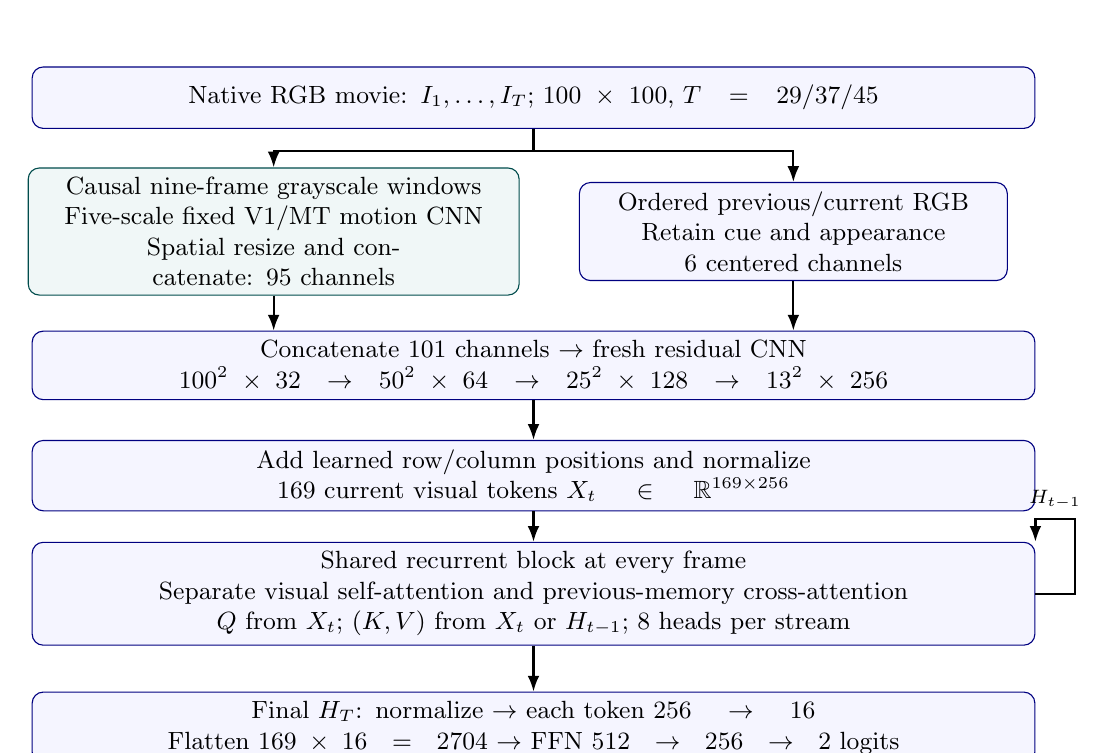
\begin{tikzpicture}[
  block/.style={draw=blue!50!black,fill=blue!4,rounded corners,align=center,font=\small,minimum height=0.78cm},
  fixed/.style={block,draw=teal!60!black,fill=teal!6},
  flow/.style={-{Latex[length=2mm]},thick},node distance=0.6cm]
\node[block,text width=12.5cm] (movie) at (0,0) {Native RGB movie: $I_1,\ldots,I_T$; $100\times100$, $T=29/37/45$};
\node[fixed,text width=6cm] (motion) at (-3.3,-1.7) {Causal nine-frame grayscale windows\\Five-scale fixed V1/MT motion CNN\\Spatial resize and concatenate: 95 channels};
\node[block,text width=5.2cm] (rgb) at (3.3,-1.7) {Ordered previous/current RGB\\Retain cue and appearance\\6 centered channels};
\node[block,text width=12.5cm] (fusion) at (0,-3.4) {Concatenate 101 channels $\rightarrow$ fresh residual CNN\\$100^2\times32\rightarrow50^2\times64\rightarrow25^2\times128\rightarrow13^2\times256$};
\node[block,text width=12.5cm] (tokens) at (0,-4.8) {Add learned row/column positions and normalize\\169 current visual tokens $X_t\in\mathbb R^{169\times256}$};
\node[block,text width=12.5cm] (memory) at (0,-6.3) {Shared recurrent block at every frame\\Separate visual self-attention and previous-memory cross-attention\\$Q$ from $X_t$; $(K,V)$ from $X_t$ or $H_{t-1}$; 8 heads per stream};
\node[block,text width=12.5cm] (readout) at (0,-8.0) {Final $H_T$: normalize $\rightarrow$ each token $256\rightarrow16$\\Flatten $169\times16=2704$ $\rightarrow$ FFN $512\rightarrow256\rightarrow2$ logits};
\draw[flow] (movie.south) -- ++(0,-0.28) -| (motion.north);
\draw[flow] (movie.south) -- ++(0,-0.28) -| (rgb.north);
\draw[flow] (motion.south) -- (fusion.north -| motion.south);
\draw[flow] (rgb.south) -- (fusion.north -| rgb.south);
\draw[flow] (fusion) -- (tokens);
\draw[flow] (tokens) -- (memory);
\draw[flow] (memory) -- (readout);
\draw[flow] (memory.east) -- ++(0.5,0) -- ++(0,0.95) -- ++(-0.5,0) node[midway,above,font=\scriptsize] {$H_{t-1}$} -- (memory.north east);
\end{tikzpicture}
\caption{Fixed motion computation supplies features; the cue, memory update and task decision are learned from the unchanged final label.}
\end{figure}

\subsection{Causal motion windows and five scales}

Let $I_t\in[0,1]^{3\times100\times100}$. We use mean grayscale $g_t=(R_t+G_t+B_t)/3$ for motion, while preserving RGB in the learned appearance path. The window available at step $t$ is
\[
  W_t=(g_{t-8},\ldots,g_t),\qquad g_s=g_1\quad\text{for }s<1.
\]
No future frame is used. Whole-movie computation is vectorized across these overlapping windows and returns one motion field per frame; the streaming interface retains eight grayscale frames.

The published image pyramid repeatedly applies its separable five-tap spatial blur and factor-two average pooling. Its five resolutions on native inputs are $100,50,25,12,6$. Time is not downsampled. The same analytic motion CNN and coefficients are shared across scales; there are not five independently trained motion estimators.

Each scale yields 19 MT channels. Spatial bilinear resizing brings each to $100\times100$ without interpolating time. Concatenating the five scale outputs yields
\[
 M_t\in\mathbb R^{95\times100\times100}.
\]
The published MT population is retained, including its zero-speed and multiple direction/speed readouts. Its velocity parameters are not newly calibrated or hand-selected for this renderer. Direction-sensitive responses at native speed were checked on gratings, but that check is not evidence of reliable native target-change classification.

\subsection{Analytic V1/MT computation}

The following equations summarize the extracted author CNN's implemented operations; the preserved source files define the coefficients. Ten separable derivative-basis channels are linearly mixed into 28 oriented V1 responses. This is an efficient implementation of directional Gaussian-derivative filtering, rather than a generic learned two-frame optical-flow network. Write
\[
 r_k = \sum_{j=1}^{10} A_{kj}(f_j*W_t),\qquad k=1,\ldots,28,
\]
where $*$ denotes the relevant space/time filtering and $A$ is fixed. If $B_{11}$ denotes the separable 11-tap spatial pooling, the V1 energy channels are
\[
 e_k=B_{11}*(r_k^2),\qquad
 v_k=\frac{e_k}{\sum_{\ell=1}^{28}e_\ell+\epsilon},\qquad \epsilon=10^{-6}.
\]
MT combines the V1 population using fixed signed coefficients $C$, applies separable 19-tap spatial pooling $B_{19}$, then rectifies, squares and normalizes:
\[
 z_a=\sum_{k=1}^{28}C_{ak}v_k,\quad
 q_a=\bigl[\max(0,B_{19}*z_a)\bigr]^2,\quad
 m_a=\frac{q_a}{\sum_{b=1}^{19}q_b+\epsilon}.
\]
The ordering matters: V1 squares before pooling; MT pools before rectification and squaring. We use the authors' CNN variant, which drops the original stage scale factors. We have not substituted the full original physiological model with its different calibration constants and normalization equation.

These operations produce population features, not a two-component optical-flow vector or a hardcoded direction decision. There are no privileged cue coordinates, target crops, event-time masks or handcoded change counters.

\subsection{Appearance fusion and spatial tokens}

At each frame the learned input is
\[
 F_t=\operatorname{concat}\bigl(I_{t-1}-\tfrac12,\ I_t-\tfrac12,\ M_t\bigr),
 \qquad I_0=I_1.
\]
Only RGB is centered; normalized motion maps are not shifted by $1/2$. Keeping RGB allows the task network to learn the visual cue and appearance information alongside movement.

The fusion CNN has a 101-to-32 stem, eight residual blocks distributed across widths 32, 64, 128 and 256, GroupNorm with eight groups, and GELU activations. Convolutions use $3\times3$ kernels and stride one. Three learned compression stages begin with pixel unshuffle, which rearranges each $2\times2$ neighborhood into channels before learned mixing. Thus spatial resolution is reduced deliberately; the model is not a full-resolution CNN throughout.

The $25\times25$ field is edge-replicated to $26\times26$ before the final compression to $13\times13\times256$. No image border is cropped. Learned row and column embeddings are added, followed by token normalization, yielding
\[
 X_t=\LN\!\left(\operatorname{reshape}(\operatorname{CNN}(F_t))+E_{\rm row}+E_{\rm col}\right)
 \in\mathbb R^{169\times256}.
\]

\subsection{Recurrent visual and memory attention}

The recurrent block is shared across frames; it is not a new transformer layer for each timestep. Let $H_0=0$ with the same shape as $X_t$, and set
\[
 Q_t=\LN_q(X_t),\qquad P_{t-1}=\LN_m(H_{t-1}).
\]
The two streams have independent learned attention projections and independent softmax normalization:
\begin{align*}
 A_t^{\rm vis}&=\MHA_{\rm vis}(Q_t,Q_t,Q_t),\\
 A_t^{\rm mem}&=\MHA_{\rm mem}(Q_t,P_{t-1},P_{t-1}),\\
 Y_t&=X_t+\frac{A_t^{\rm vis}+A_t^{\rm mem}}{\sqrt2},\\
 H_t&=Y_t+\operatorname{FFN}(\LN_f(Y_t)).
\end{align*}
Each stream has eight heads of width 32. The FFN is $256\rightarrow1024\rightarrow256$ with GELU. The current visual representation queries the previous memory; the implementation does not concatenate both sources into one shared key/value softmax. Keeping separate normalization permits both sources to contribute without directly competing within a single attention distribution.

Memory has a fixed 169-token extent. There is no growing frame cache, CLS token, GRU, second KDA arm or explicit phase-dependent retention gate. Information preservation must be learned through the existing recurrent computation; the motion front end does not guarantee it.

\subsection{Final spatial readout and parameter accounting}

Only the final memory state contributes to the supervised decision:
\[
 U=\GELU(W_{16}\LN_r(H_T)+b_{16}),\qquad
 U\in\mathbb R^{169\times16}.
\]
Flattening preserves token identity. The classifier is $2704\rightarrow512\rightarrow256\rightarrow2$, with GELU between its linear layers. We do not average away left/right spatial distinctions before the response.

\begin{center}
\begin{tabular}{lr}
\toprule
Learned component & Parameters \\
\midrule
Fusion CNN & 4,715,616 \\
Row and column positions & 6,656 \\
Token normalization & 512 \\
Recurrent visual block & 1,053,440 \\
Final readout normalization & 512 \\
Token projection $256\rightarrow16$ & 4,112 \\
Classifier & 1,516,802 \\
\midrule
Total learned parameters, 92 tensors & \textbf{7,297,650} \\
Fixed analytic buffer values & 2,430 \\
\bottomrule
\end{tabular}
\end{center}

Every learned parameter starts fresh and remains trainable. The fixed front end uses published analytic coefficients as mathematical buffers; no trained segmentation checkpoint or previous project model is loaded. This distinction is deliberate: the hypothesis concerns a supplied motion computation, with a freshly learned cue/memory/decision pathway.

\section{Source adaptations and local execution}

\textbf{Source.} We preserve the original author files and extract only the needed classes, avoiding unrelated MMFlow dependencies. The repository commit is \code{997ec55adf6062d8f92d4adcd555fdaccc5a1200}. This is an adaptation of the published motion estimator, not an end-to-end reproduction of their segmentation system.

\textbf{Coefficient layout.} The original analytic factory stores the three separable V1 filter tensors in H,W,T layout, whereas the extracted CNN consumes T,H,W. The wrapper permutes those tensors once. Every coefficient and sign is preserved; the upstream files remain unchanged.

\textbf{Causal alignment.} The nine-tap temporal filter is evaluated over past-eight-plus-current windows. Relative to its centered alignment, its nominal midpoint is four frames earlier than the current output, a 40 ms shift at the native clock. Its complete support covers eight frame intervals. This delay may matter for a short post-event segment. We neither expose future frames nor append extra task frames to compensate. Startup repeats only the first image.

\textbf{Task head.} The published coarse-to-fine segmentation head is replaced by our spatial fusion CNN, RViT and binary response decoder. Mean grayscale conversion and spatial concatenation are part of this task adapter. No auxiliary motion labels or segmentation supervision have been introduced.

\textbf{Apple backend.} All learned computation runs in FP32 on the local M4 Max's MPS device. The analytic front end runs in FP32 on CPU with two threads. The native MPS path lacks \code{avg_pool3d.out}; replacing only that pool with equivalent per-frame 2D pooling permitted execution but yielded material CPU/MPS differences after channel normalization on a random movie (maximum absolute difference approximately 0.164). We therefore retained the unchanged CPU analytic computation rather than using that numerically discrepant path. The CPU-to-MPS copies remain differentiable, and do not truncate gradients through the learned recurrent model.

The runtime is source-isolated outside the Desktop workspace at \code{/Users/jonathanmorgan/VAWMRuntime/structured_motion_rvit_local01}. Its production model, optimizer, random states and native streams were initialized anew after disposable profiling. Earlier artifacts remain preserved.

\section{Training protocol now running}

\subsection{Trial replay and whole-sequence updates}

The latest user-selected policy is retained: generate 1,000 native trials, train for ten shuffled epochs over that pool, then replace it with 1,000 fresh trials while retaining the learned model and Adam state. The first pool has 334 B12, 333 B20 and 333 B28 movies; the extra trial rotates across conditions in later pools.

Because lengths differ, batches are homogeneous by condition. Each epoch shuffles examples within each condition and shuffles the condition order within successive batch rounds. Each condition contributes ten full batches of 32 plus one tail of 13 or 14, giving 33 updates per epoch and 330 updates per pool. All 1,000 trials are used exactly once per epoch. Tail updates use their actual example count when normalizing loss.

The effective batch is 32, accumulated as one complete trial at a time. For a batch of actual size $n$,
\[
 \mathcal L=\frac1n\sum_{i=1}^n-\log\operatorname{softmax}(\ell(I_{1:T}^{(i)}))_{y_i}.
\]
Each trial processes its whole native movie, with one final binary cross-entropy contribution, then backpropagates through every recurrent step. One Adam step follows the accumulated batch. Parameters stay fixed throughout those trial forward/backward passes. There is no per-frame optimizer update, truncated BPTT, detached memory, teacher forcing or intermediate-frame supervision. Memory and raw-frame history reset between trials. Encoder activation checkpointing saves memory by recomputing learned spatial activations on backward.

\begin{center}
\begin{tabular}{ll}
\toprule
Setting & Executed policy \\
\midrule
Optimizer & Adam, one parameter group \\
Learning rate & $10^{-4}$ \\
Betas; epsilon & $(0.9,0.999)$; $10^{-8}$ \\
Weight decay; clipping & 0; none \\
Precision; temporal gradients & FP32; full BPTT \\
Batch / microbatch & 32 / 1, with actual-size tails \\
Model and optimizer initialization & Fresh; no profile/predecessor state \\
CPU bound & Two threads \\
Evaluation microbatch & One whole trial \\
\bottomrule
\end{tabular}
\end{center}

\subsection{Measured allocation and deadlines}

We discarded a three-condition warmup cycle and measured three further full-batch updates, one per native length, plus 20 evaluation trials per condition. The measured optimizer allocation for two complete pools is approximately 16,452 seconds; conservative planning includes timing margins, validation, two final tests and reporting.

The prospective allocation is \textbf{660 updates / 20,000 presentations / 2,000 unique movies}. It completes two ten-epoch pools. These counts must not be described as 20,000 independent fresh movies. The prospective ceiling of 4,216 updates was reduced before production to what complete pools fit within the finite local allocation.

The cap is eight hours, conservatively retaining the first compatibility-attempt timestamp: 2 October at 6:15:49 PM PDT. The scientific cutoff is 3 October at 2:05:49 AM PDT; the independent hard guard stops this job by 2:15:49 AM PDT. Setup, profiling, training, evaluation and reporting share the cap. There is no automatic renewal or extra training arm.

\subsection{Validation, selection and decision criteria}

Validation is scheduled at updates 100, 250, 500 and 660, using 100 fresh evaluation trials per condition from separate validation streams. Selection maximizes mean three-condition AUC, then mean balanced accuracy, with the earlier checkpoint retained on ties. Checkpoints are also saved every 100 updates and at startup and termination.

Fresh final tests use 200 trials per condition for the selected and terminal checkpoints, with paired draws between these two evaluations. Report each condition's balanced accuracy and AUC, target hit rate, foil false-alarm rate and catch false-positive rate. Live validation snapshots remain distinct from final held-out tests. A positive-only response can achieve the label prior while still yielding 50\% balanced accuracy; the loss alone is insufficient evidence of task learning.

The inherited provisional reporting thresholds are balanced accuracy of at least 70\% in every native condition for acquisition, and at least 90\% in every condition for the working solved-task target. These thresholds do not select checkpoints, alter stimuli or stop a healthy run early. Subgroup results remain necessary to understand what behavior was acquired; finite tests and one fresh initialization do not establish biological equivalence or universal generalization.

\section{Evidence at launch and proposal for interpretation}

\textbf{Completed implementation checks.} Three focused CPU checks passed: analytic coefficient/layout parity and causal streaming equivalence; opposite-direction gratings at 0.375 pixels/frame produce different motion populations; a native 29-frame movie gives finite logits and the short gradient check reaches every learned tensor and the earliest input frame. The chosen CPU-front-end/MPS-learner path additionally completed a native 29-frame backward pass with finite gradients for all 92 learned tensors and motion features bitwise equal to the CPU reference. These checks establish implementation readiness, not acquired task performance.

\textbf{Actual training evidence.} Fresh production checkpoint 3 was independently reloaded on CPU at approximately 6:30 PM PDT. It contains 96 presented trials, all 92 Adam states at step 3, and changes in every learned parameter tensor. The initial checkpoint equals direct fresh construction with an empty optimizer and fresh streams. All analytic buffer values are unchanged. At that checkpoint the B12 batch loss was approximately 0.677; no production validation had yet occurred. This is a launch snapshot, not a current progress claim.

\textbf{Replacement of the old local run.} The previous delayed-frame CNN--GRU was stopped at the user's request and saved at 2,575 updates / 82,400 fresh trials. Its weights and optimizer remain preserved; they are not inputs to this candidate. No final-test claim is made for the cancelled run. Existing cloud runs retain their own unchanged allocations.

\textbf{Decision after this run.} If fresh final performance clears the acquisition threshold across all three conditions, this candidate is a useful architecture from which to continue development. If it reaches the working solved-task target with credible target/foil/catch behavior, inspect generalization and seed robustness before broader claims. If it remains near chance, the result narrows this particular fixed-front-end-plus-RViT proposal; it does not show that neural networks cannot solve the task or that motion information is absent.

Any gain is evidence for the complete architecture and training package. The motion front end changes both representation and temporal support, and the learned fusion stem has additional input channels. The cancelled CNN--GRU also used a different fresh-sampling policy, while the cloud replay RViT has different hardware and exposure. These runs supply context and learning curves, but they are not a matched intervention that uniquely attributes an improvement to a physiological motion mechanism. No new diagnostic or training arm is automatically launched by this proposal.

\section{Implementation and primary references}\label{sec:references}

\textbf{Implementation files.} Paths are relative to the project root.
\begin{itemize}
\item \code{SecondPass/StructuredMotionRViT/model.py}: fixed motion adapter, fresh fusion encoder and RViT.
\item \code{SecondPass/StructuredMotionRViT/author_cnn.py}: extracted author classes.
\item \code{SecondPass/StructuredMotionRViT/upstream/}: original sources, configuration and source hashes.
\item \code{SecondPass/StructuredMotionRViT/worker.py}: replay training adapter and measured local allocation.
\item \code{SecondPass/StructuredMotionRViT/LocalRuntime/}: launch, guard and independently reloaded production receipt.
\item \code{SecondPass/StructuredMotionRViT/verification/}: focused CPU and mixed CPU/MPS evidence.
\end{itemize}

\textbf{Primary sources.}
\begin{enumerate}
\item Tangemann, M., K\"ummerer, M., and Bethge, M. (2024). \emph{Object segmentation from common fate: Motion energy processing enables human-like zero-shot generalization to random dot stimuli}. NeurIPS 37. \href{https://papers.nips.cc/paper_files/paper/2024/file/f7d3cef7ff579f2f903c8f458e730cae-Paper-Conference.pdf}{Paper PDF}; \href{https://github.com/mtangemann/motion_energy_segmentation}{official implementation}.
\item Simoncelli, E. P., and Heeger, D. J. (1998). \emph{A Model of Neuronal Responses in Visual Area MT}. Vision Research 38(5), 743--761. \href{https://www.cns.nyu.edu/pub/eero/simoncelli96-reprint.pdf}{Author-hosted paper}; \href{https://www.cns.nyu.edu/~lcv/MTmodel/}{original model and software}.
\item Arcizet, F., and Krauzlis, R. J. (2018). \emph{Covert spatial selection in primate basal ganglia}. PLOS Biology. \href{https://doi.org/10.1371/journal.pbio.2005930}{Primary task source}. The current native renderer's disclosed adaptations remain unchanged.
\end{enumerate}

\end{document}
